\subsection{What is the Value of a Model Based on Average Feature Values?}
\label{sec:mean-model}
I am not the first to observe that fitting a model to the mean of feature values across a distribution of cells of the same type may not result in a model that well-described an actual neuron from that distribution.
Neuron modelers have some awareness of this problem which has been thoroughly characterized in \cite{marder2011multiple}, though it remains underappreciated.
This is especially obvious when the feature distribution is multi-modal (such as inset-e in the figure below), but it could also result from hidden covariance structure among the features (Figure \ref{fig:eve_marder}).

\begin{figure}
\begin{center}
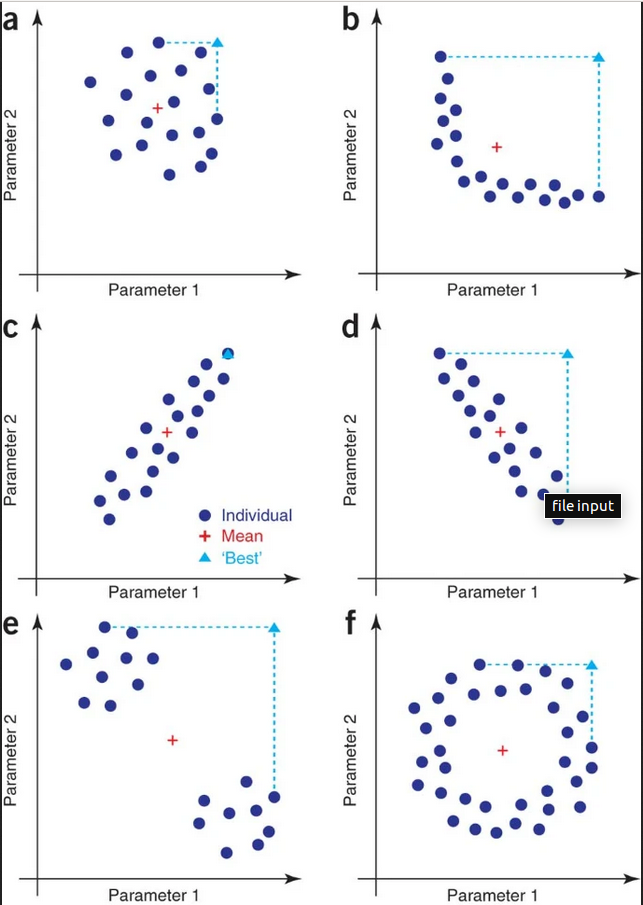
\includegraphics[scale=0.65]{figures/eve_marder.png}
\end{center}
\caption[Considerations from Marder]{\textbf{Lessons from Marder.} As shown in \cite{marder2011multiple}, when neurons of a given type are distributed through parameter space, the mean of these parameters across neurons (red cross) is at a separate location from the model one would obtain by using different neurons to contrain different parameters (blue triangle).}
\label{fig:eve_marder}
\end{figure}

Previously in the Methods (Section \ref{sec:neuroelectro}), we showed that some feature distributions are bimodal.
Consider a cell type which had an underlying bimodal distribution for input resistance, with a mean exactly between the two modes.
If we optimize a neuron against this mean value, then the optimized neuron does not describe the modes (where most of the cells are actually located) at all.
Conversely, suppose that we optimize each neuron from the distribution individually, and then produce a model which just averages across the parameter values of each of these optimized models.
Its entirely conceivable that that this ``mean model" would produce measurements that were similar to the mean of the feature distribution.
However, when we are dealing with a nonlinear dynamical system, this is by no means certain (and perhaps not even likely).
This mean model could also exhibit much higher or lower feature values.
For example, we expect that even these comparatively simple reduced models have multiple regimes characterized by sharp transitions in parameter space between, for example, regular spiking behavior and bursting behavior, or tonic-bursting vs chattering.
What would it even mean to split the difference between two such fundamentally different regimes?

In order to examine this question further in the context of my optimizer applied to reduced models, I created two models from each model class (e.g. Izhikevich) with different sets of parameter values.
I simulated each of these models, computed all of the measurements associated with the core NeuronUnit tests (rheobase, input resistance, capacitance, and membrane time constant), and then simply averaged them together across the two models.
I call these the ``mean features" as each one reflects the mean across two parameterizations of the model.
In parallel, I also create a ``mean model" (Figure \ref{fig:mean-model-polar}) which reflects the average of the parameters themselves, and then measure the same set of features for this mean model.
I then ask the question: "Do the features from the mean model match the mean features?"
If these match nearly all of the time, we can feel confident that optimizing a model based on the mean features will produce a model that is representative of the parameter space of the neurons individually.
In other words, if we had access to the measurements from the individual neurons, and fit models to those, then the mean model obtained above should lie somewhere between those models in parameter space.
By contrast, if the mean model does not match the mean features, that would suggest that models obtained by optimizing against mean features may not be representative in this context.

The results are shown below.
In Figure \ref{fig:mean-model-polar}, I show a representative example using two random locations in parameter space.
While some of the differences between the two parameter sets may look small, this is only a reflection of the scale being dominated by the parameters that intrinsically have the largest values.

\begin{figure}
\begin{center}
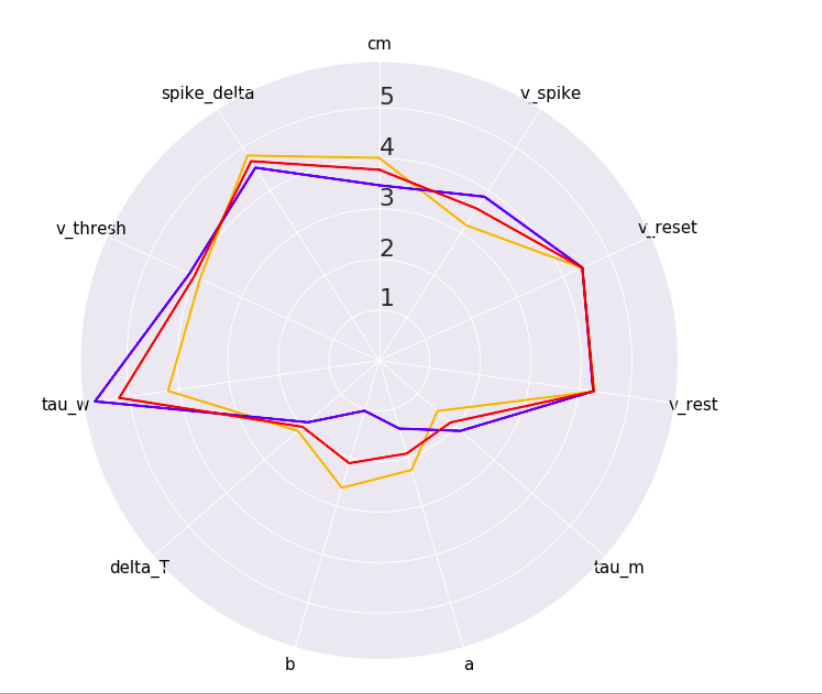
\includegraphics[]{figures/polar_coordinates.png}
\caption[Mean of Random Models]{\textbf{Construction of a Model from the Mean.}
Two random AdEx models (yellow and purple traces) are drawn from multivariate uniformly distributed random number generators.
The mean model (red trace) is defined as the location in parameter space exactly in between the two random models in every dimension.
Logarithms and absolute values are used to scale the radial dimension for clarity.}
\label{fig:mean-model-polar}
\end{center}
\end{figure}


%\begin{table}
%\begin{adjustbox}{width=\columnwidth,center}
%\begin{tabular}{lrrrrrrrrrrr}
%\toprule {} &          cm &    v\_spike &    v\_reset &     v\_rest &      tau\_m &         a &          b &   delta\_T &       tau\_w &   v\_thresh &  spike\_delta \\
%\midrule
%a           &  954.283985 & -39.652421 & -33.290058 & -71.274552 &  18.409430 &  8.732663 &  13.449849 &  9.178972 &  205.178522 & -29.526272 &    69.811681 \\
%b           &  885.614383 & -57.290057 & -57.805723 & -96.183985 &  51.917341 &  0.086329 &  13.464095 &  8.315697 &  271.050894 & -58.339164 &    93.170984 \\
%mean of a and b &  919.949184 & -48.471239 & -45.547891 & -83.729269 &  35.163385 &  4.409496 &  13.456972 &  8.747335 &  238.114708 & -43.932718 &    81.491333 \\
%\bottomrule
%\end{tabular}
%\end{adjustbox}
%\caption[coordinate information in tabular form]{The same polar coordinates in tabular form.}
%\end{table}

I then compute an index of agreement between features derived from the mean model vs mean features observed across the original two models.
This index, $\alpha=\lvert\frac{(x-a)}{(b-a)}\rvert$, where $a$ and $b$ are the feature values for the original two models, and $x$ is the feature value for the mean model, can be interpreted as follows:
If $\alpha=0.5$, then the mean model produces features precisely in between those produced by the two original models (Figure \ref{fig:mean-model-3}).
If $\alpha=0$ or $\alpha=1$, then the mean model is nearly identical (in that feature) to one of the original models.
An example of values ranging between 0 and 1 is shown in Figure \ref{fig:mean-model-4}.
If $\alpha>1$, then the mean model produces entirely new feature values that would not be expected from an interpolating between the two original models.

\begin{figure}
    \centering
    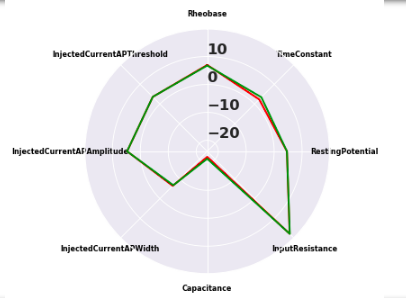
\includegraphics{figures/model_similarities.png}
    \caption[Example of Mean Model Versus Mean Feature Agreement]{\textbf{Example of Mean Model vs Mean Feature Agreement}.
    Two random models can produce feature values whose mean (green) is equal to the feature values (red) produced by a model defined by the mean of their parameters.
    In such case the index of agreement $\alpha=0.5$.}
    \label{fig:mean-model-3}
\end{figure}

\begin{figure}
    \centering
    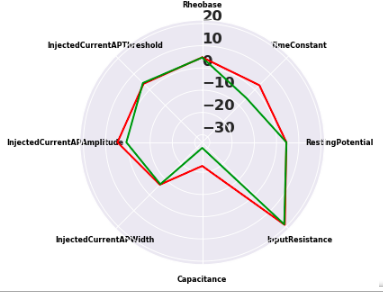
\includegraphics{figures/model_differences.png}
    \caption[Example of Mean Model Versus Mean Feature Disagreement]{\textbf{Example of Mean Model vs Mean Feature Disagreement.} Similar to Figure \ref{fig:mean-model-3}, but now showing several disagreements, between mean model and mean feature value (in Capacitance, Time Constant, and AP Amplitude).}
    \label{fig:mean-model-4}
\end{figure}

Figures \ref{fig:mean-model-1} and \ref{fig:mean-model-2} show that, while $\alpha=0.5$ is the mode of the distribution as might be expected, considerable mass lies outside the mode, including many values of $\alpha>1$.
Therefore any model optimized against the mean feature value across neuron cannot be equivalent to a model drawn from the mean of those neurons' multivariate parameter distribution.

\begin{figure}
    \centering
    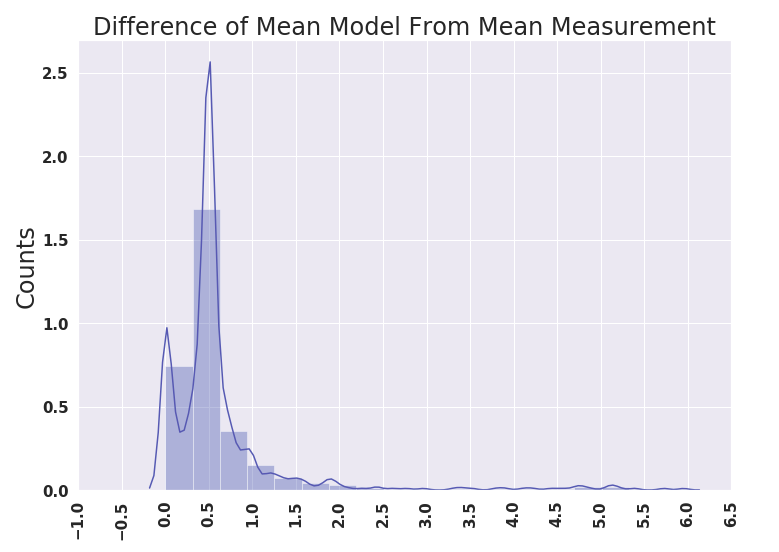
\includegraphics{figures/mean_model_vs_mean_measurement.png}
    \caption[Mean Model Versus Mean Features for AdEx Model]{\textbf{Mean Model vs Mean Features for AdEx Model.} For 100 pairs of randomly sampled AdEx models, I computed the index $\alpha$ of mean model vs mean feature agreement, defined (see text) such that a value of 0.5 indicates that the mean model produces features identical to those obtained by simply averaging feature values produced by the original models.
    The mode lies at $~0.5$, but density in other regions indicates that many mean models do not agree with the mean feature value.}
    \label{fig:mean-model-1}
\end{figure}

\begin{figure}
    \centering
    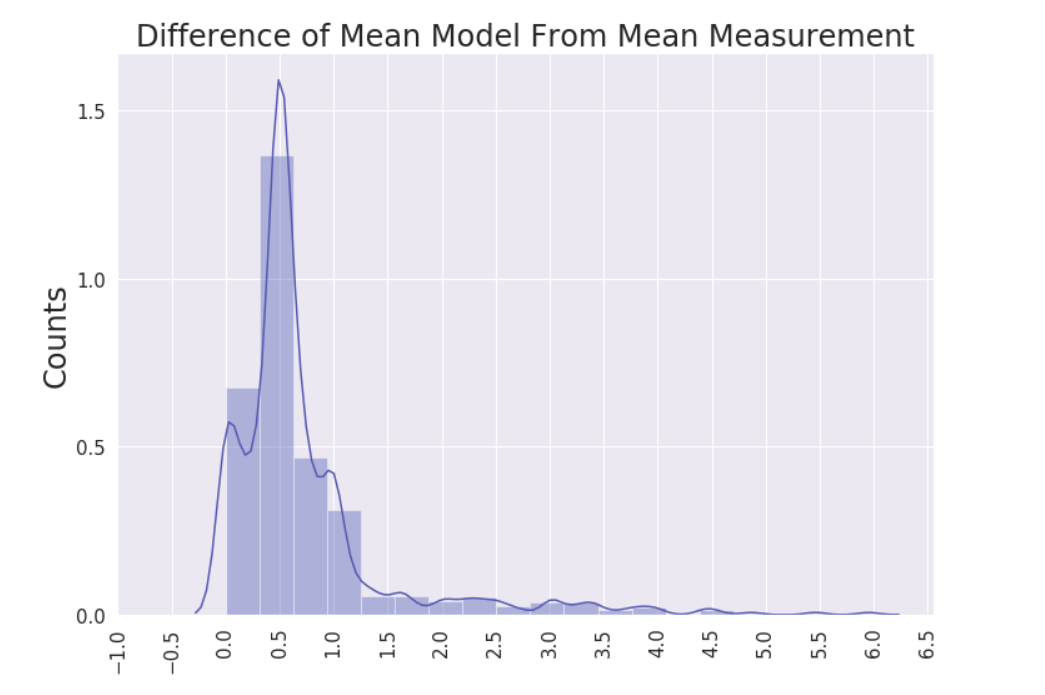
\includegraphics{figures/reproduced_izhi.png}
    \caption[Mean Model Versus Mean Features for Izhikevich Model]{\textbf{Mean Model vs Mean Features for the Izhikevich Model.} Same as Figure \ref{fig:mean-model-1}, but for the Izhikevich model.}
    \label{fig:mean-model-2}
\end{figure}

%\begin{figure}
%    \centering
%    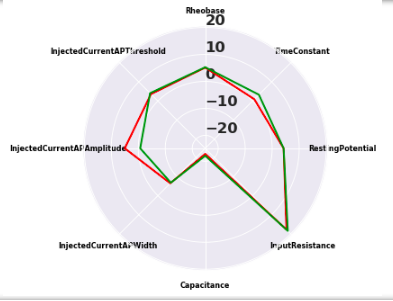
\includegraphics{figures/model_differences2.png}
%        \label{fig:mean-model-5}
%    \caption[Second example of disparity in mean model, mean measurement agreement]{This time I show a less common pattern of disagreement, between mean model and mean measurement.}
%\end{figure}


%\begin{figure}
%    \centering
%    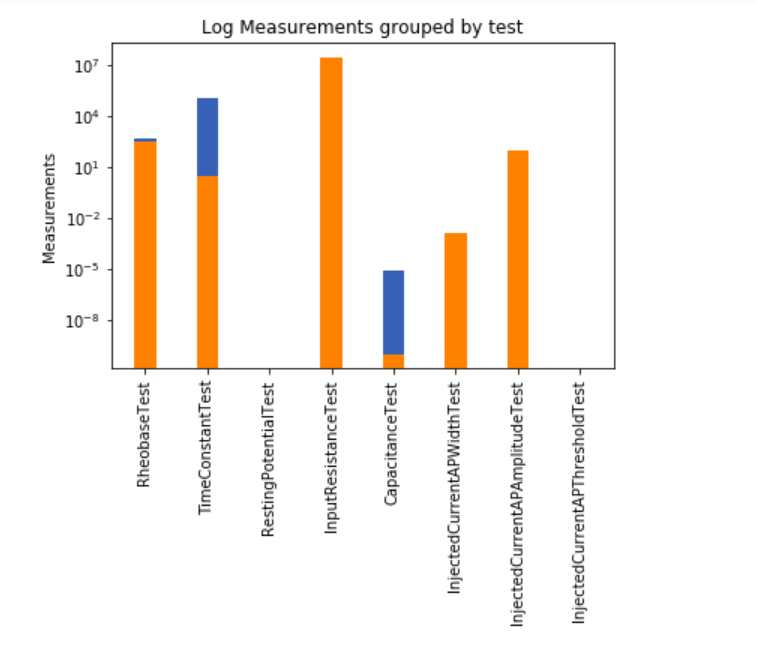
\includegraphics{figures/mean_model_mean_test.png}
%    \caption{Caption}
%    \label{fig:my_label}
%\end{figure}

In Figures \ref{fig:mean-model-3} and \ref{fig:mean-model-4}, I show the computed feature values from simulations of the constructed as in Figure \ref{fig:mean-model-polar}.
While in some cases the mean model produces feature values that lie between (are equal to the mean of) the feature values of the original two models, in other cases there is a massive discrepancy.
This discrepancy appears more common in the Izhikevich model than in the AdEx model, potentially because there is a greater likelihood that the two original random models describe different dynamical regimes.

%Although the peak identified in Figure \ref{fig:mean-model-2} looks taller in absolute size compared to Figure \ref{fig:mean-model-1}, the scale along the y-axis is different.
%Figure \ref{fig:mean-model-1} exhibits more histogram counts at 0.5, i.e. the mean model was more likely to exhibit features very similar to the mean features of the two models.

During the course of this work I observed that generally the mapping between reduced model parameters space and the feature space is not isomorphic, and thus fitting models to the mean feature values for a distribution of neurons is a dangerous exercise even if the data are normal-like.

%\begin{figure}
%    \centering
%    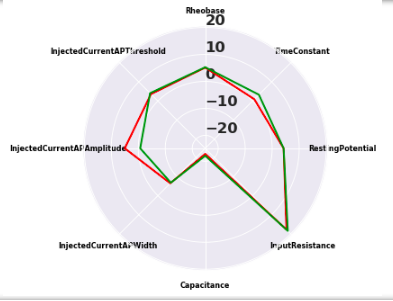
\includegraphics{figures/model_differences2.png}
%        \label{fig:mean-model-1}
%    \caption[Second example of disparity in mean model, mean measurement agreement]{This time I show a less common pattern of disagreement, between mean model and mean measurement.}
%\end{figure}

%\begin{comment}
%\begin{figure}
%    \centering
%    \includegraphics{figures/mean%_model_mean_test2.png}
%    \caption[bar charts that reveal disparity between mean model and mean measurement]{A stacked bar chart was used and each bar was positioned to represent each of the different measurement types. Very often the mean model measurement, green, is at a comparable height as model a, b and the mean model. There are two glaring exceptions which are the time constant measurement, and the capacitance measurement. At those measurement locations the mean is significantly greater than the mean of model a and model b}
%    \label{fig:mean-model-2}
%\end{figure}
%\end{comment}

%explore if this was a problem for models as well as experimental cells.